\documentclass{beamer}
\usetheme{Boadilla}
\usecolortheme{sidebartab}
\beamertemplatenavigationsymbolsempty
\setbeamertemplate{footline}[frame number]
\usepackage{hyperref} 
\usepackage{graphicx}
\usepackage{color}
\usepackage{booktabs}
\usepackage{listings}
\usepackage{soul}
\usepackage{tikz}
\usepackage[utf8]{inputenc}
\usepackage{CJKutf8}
\usetikzlibrary{shapes.geometric}

\definecolor{gray}{rgb}{0.4,0.4,0.4}
\definecolor{darkblue}{rgb}{0.0,0.0,0.6}
\definecolor{cyan}{rgb}{0.0,0.6,0.6}

\lstset{
	basicstyle=\ttfamily,
	columns=fullflexible,
	showstringspaces=false,
	commentstyle=\color{gray}\upshape
}

\tikzset{node style/.style={
		draw=blue,
		thick,
		fill=blue!70,
		text=white,
		ellipse,
		minimum width=2cm,
		minimum height=0.75cm,
		font=\small,
		outer sep=3pt,
	},
	blank style/.style={
		draw=black,
		thick,
		fill=white,
		text=white,
		ellipse,
		minimum width=2cm,
		minimum height=0.75cm,
		font=\small,
		outer sep=3pt,
	},
	literal style/.style={
		draw=red,
		thick,
		fill=red!70,
		text=white,
		rectangle,
		minimum width=2cm,
		minimum height=0.75cm,
		font=\small,
		outer sep=3pt,
	},
	edge style/.style={
		#1,
		text=black,
		font=\footnotesize,
		above
	}
}

\makeatletter
\newcommand\SoulColor{%
	\let\set@color\beamerorig@set@color
	\let\reset@color\beamerorig@reset@color}
\makeatother

\lstset{language=XML}

\title{RDF Syntax: Eine Breite Wahl}
\author{Markus Stocker}
\date{30. April 2018}

\begin{document}

\maketitle

\begin{frame}{Rekapitulation}
	
	\begin{itemize}
		\item Woraus besteht ein \emph{statement}?
		\item Was ist ein URI und wozu dient dieser in RDF?
		\item Wie entstehen RDF Graphen?
		\item Welche Vorteile haben RDF Graphen gegenüber XML Bäume?
	\end{itemize}
	
\end{frame}

\begin{frame}{Übersicht}
	
	\begin{itemize}
		\item Graph Darstellung
		\item Das Tripel
		\item Serialisierung
		\item RDF Syntaxen
	\end{itemize}
	
\end{frame}

\begin{frame}{Graph Darstellung}
	
	\begin{itemize}
		\item In der letzten Vorlesung haben wir Graphen visuell dargestellt
		\item Solche Darstellung ist einfach in der kommunikation mit Menschen
		\item Geeignet für Vorlesungen, Folien und kleine Graphen
		\item Allerdings klar ungeignet für Maschinenverarbeitung
		\item Auch nicht geeignet für grosse Graphen
	\end{itemize}
	
\end{frame}

\begin{frame}{Graph Darstellung}
	
	\begin{itemize}
		\item Für maschinelle Verarbeitung benötigen wir eine Serialisierung
		\item Transformation eines Graphen in eine Zeichenfolge
		\item Letztlich ein Text Dokument (Datenbank für grössere Datenmengen)
		\item Ähnlich wie Serialisierung von XML Bäume als Text Dokumente
	\end{itemize}
	
\end{frame}

\begin{frame}{Von Graphen zu Tripelmengen}
	
	\begin{itemize}
		\item Graph kann man anhand der Kanten zerlegen
		\item Jede Kante mit verknüpften Knoten ist eindeutig
		\item Zwei über eine Kante verknüpfte Knoten ist Elementareinheit
		\item In RDF wird diese Einheit Tripel (\emph{triple}) genannt
		\item Ein RDF Graph ist somit eine Tripelmenge
		\item Und zwar ungeordnete Menge
	\end{itemize}
	
\end{frame}

\begin{frame}[fragile]{Das Tripel}
	
	\begin{itemize}
		\item Ein Triple besteht aus Subjekt, Prädikat, und Objekt
	\end{itemize}
	
	\begin{lstlisting}
	Triple := (Subject, Predicate, Object)
	\end{lstlisting}
		
	\begin{itemize}
		\item Prädikate entsprechen Graph Kanten
		\item Üblicherweise mit \texttt{p} gekürzt
		\item Prädikate zeigen immer vom Subjekt zum Objekt
	\end{itemize}
	
	\centering
	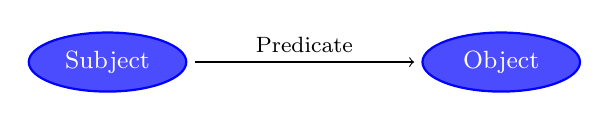
\begin{tikzpicture}[node distance=5cm]
		\node[node style] (s) {Subject};
		
		\node[node style, right of=s] (o) {Object}
		edge [<-] node[edge style=sloped,above]{Predicate} (s);
	\end{tikzpicture}
	
	\begin{itemize}
		\item Subjekt und Objekt entsprechen Graph Knoten
		\item Üblicherweise jeweils mit \texttt{s} und \texttt{o} gekürzt
	\end{itemize}
	
	\begin{lstlisting}
	Triple := (s, p, o)
	\end{lstlisting}
	
\end{frame}

\begin{frame}{Das Tripel}
	
	\begin{itemize}
		\item Prädikate sind mittels URI immer benannt
		\item Subjekt und Objekt können unbenannt sein (\emph{blank node})
		\item Subjekt und Objekt können mittels URI benannt sein
		\item Objekt kann ein Literal sein
	\end{itemize}
	
\end{frame}

\begin{frame}{Tripel Syntaxen}
	
	\begin{itemize}
		\item Es gibt mehrere Syntaxen für Tripelmengen
		\item N-Triples, Turtle, und RDF/XML wohl die bekanntesten
		\item Es handelt sich um drei Serialisierungen 
		\item Für Tripelmengen (RDF Graphen) nach RDF (Text) Dokumente
		\item Jede Syntax hat Vor- und Nachteile
		\item Es ist möglich zwischen Syntaxen zu konvertieren
		\item Konvertierung ohne Informationsverlust
	\end{itemize}
	
\end{frame}

\begin{frame}{N-Triples}
	
	\begin{itemize}
		\item Zeilenorientierte Serialisierung einer Tripelmenge
		\item Einfach für Software zu lesen und schreiben
		\item Ideal für \emph{streaming} Anwendungen
		\item Ein Tripel endet mit einem Punkt
		\item Jedes Tripel meist auf eigener Zeile (nicht zwingend)
		\item Leerzeichen und Umbrüche ausserhalb URI und Literal ignoriert
		\item URIs zwischen spitze Klammern 
		\item Literale zwischen Anführungszeichen
	\end{itemize}
	
\end{frame}

\begin{frame}[fragile]{N-Triples: Beispiel}
	
	\scriptsize
	\begin{lstlisting}
<http://example.org#Earth> <http://www.w3.org/2000/01/rdf-schema#label> "Earth" .
<http://example.org#Earth> <http://www.w3.org/2000/01/rdf-schema#label> "Erde" .
<http://example.org#Earth> <http://www.w3.org/2000/01/rdf-schema#label> "Terra" .
<http://example.org#Earth> <http://example.org#radius> "6371.0" .
	\end{lstlisting}
	
\end{frame}

\begin{frame}[fragile]{N-Triples: \emph{Blank Node}}
	
	\small
	\begin{lstlisting}
<http://example.org#Earth> <http://example.org#radius> _:b .
_:b <http://example.org#value> "6371.0" .
_:b <http://example.org#unit> <http://units.org#km> .
	\end{lstlisting}
	
\end{frame}

\begin{frame}{Turtle}
	
	\begin{itemize}
		\item Eine Obermenge von N-Triples
		\item Führt Präfixe ein um URIs zu kürzen
		\item Bei gleichem Subjekt (und Prädikat) kann URI entfallen
		\item Einfach für Menschen zu lesen, kompakt
		\item Für Maschinen wird entsprechender Parser benötigt
	\end{itemize}
	
\end{frame}

\begin{frame}[fragile]{Turtle: Beispiel}
	
	\small
	\begin{lstlisting}
  @prefix ex: <http://example.org#> .
  @prefix rdf: <http://www.w3.org/1999/02/22-rdf-syntax-ns#> .
  @prefix rdfs: <http://www.w3.org/2000/01/rdf-schema#> .

  ex:Earth rdf:type ex:Planet ;
            rdfs:label "Earth", "Erde", "Terra" ;
            ex:radius "6371.0" .
	\end{lstlisting}
	
\end{frame}

\begin{frame}[fragile]{N-Turtle: \emph{Blank Node}}
	
	\small
	\begin{lstlisting}
  @prefix ex: <http://example.org#> .
  @prefix rdf: <http://www.w3.org/1999/02/22-rdf-syntax-ns#> .
  @prefix rdfs: <http://www.w3.org/2000/01/rdf-schema#> .
  @prefix unit: <http://units.org#> .
	  
  ex:Earth rdf:type ex:Planet ;
            rdfs:label "Earth", "Erde", "Terra" ;
            ex:radius [
              ex:value "6371.0" ;
              ex:unit unit:km
            ] .
	\end{lstlisting}
	
\end{frame}

\begin{frame}{RDF/XML}
	
	\begin{itemize}
		\item XML basierte RDF Serialisierung
		\item Weit verbreitet, XML Parser in vielen Programmiersprachen
		\item Triple Gruppierung anhand Subjekte
		\item Wurzelknoten ist \texttt{rdf:RDF} mit globalen Namensräumen
	\end{itemize}
	
\end{frame}

\begin{frame}[fragile]{RDF/XML: Beispiel}
	
	\footnotesize
	\begin{lstlisting}
  <rdf:RDF xmlns:rdf="http://www.w3.org/1999/02/22-rdf-syntax-ns#"
            xmlns:rdfs="http://www.w3.org/2000/01/rdf-schema#"
            xmlns:ex="http://example.org#">
	
    <rdf:Description rdf:about="http://example.org#Earth">
      <rdf:type rdf:resource="http://example.org#Planet"/>
      <rdfs:label>Earth</rdfs:label>
      <rdfs:label>Erde</rdfs:label>
      <rdfs:label>Terra</rdfs:label>
      <ex:radius>6371.0</ex:radius>
    </rdf:Description>
	
  </rdf:RDF>		
	\end{lstlisting}
	
\end{frame}

\begin{frame}[fragile]{RDF/XML: \emph{Blank Node} (1)}
	
	\small
	\begin{lstlisting}
  <rdf:RDF xmlns:rdf="http://www.w3.org/1999/02/22-rdf-syntax-ns#"
            xmlns:rdfs="http://www.w3.org/2000/01/rdf-schema#"
            xmlns:ex="http://example.org#">
    
    <rdf:Description rdf:about="http://example.org#Earth">
      <rdf:type rdf:resource="http://example.org#Planet"/>
      <ex:radius>
        <rdf:Description>
          <ex:value>6371.0</ex:value>
          <ex:unit rdf:resource="http://units.org#km"/>
        </rdf:Description>
      </ex:radius>
    </rdf:Description>
    
    </rdf:RDF>
	\end{lstlisting}
	
\end{frame}

\begin{frame}[fragile]{RDF/XML: \emph{Blank Node} (2)}
	
	\small
	\begin{lstlisting}
  <rdf:RDF xmlns:rdf="http://www.w3.org/1999/02/22-rdf-syntax-ns#"
            xmlns:rdfs="http://www.w3.org/2000/01/rdf-schema#"
            xmlns:ex="http://example.org#">
	
    <rdf:Description rdf:about="http://example.org#Earth">
      <rdf:type rdf:resource="http://example.org#Planet"/>
      <ex:radius rdf:nodeID="_:b"/>
    </rdf:Description>
	
    <rdf:Description rdf:nodeID="_:b">
      <ex:value>6371.0</ex:value>
      <ex:unit rdf:resource="http://units.org#km"/>
    </rdf:Description>
	
  </rdf:RDF>
	\end{lstlisting}
	
\end{frame}

\begin{frame}[fragile]{RDF/XML: \texttt{rdf:ID} und \texttt{rdf:about}}
	
	\begin{itemize}
		\item Anstatt \texttt{rdf:about} kann auch \texttt{rdf:ID} benutzt werden
		\item Allerdings darf \texttt{rdf:ID} für ein URI nur einmal verwendet werden
    \end{itemize}
   
   	\small
   	\begin{lstlisting} 
  <rdf:RDF xmlns:rdf="http://www.w3.org/1999/02/22-rdf-syntax-ns#"
            xmlns:ex="http://example.org#"
            xml:base="http://example.org">
    
    <ex:Planet rdf:ID="Earth"/>
    
    <ex:Planet rdf:about="#Mars"/>
    
  </rdf:RDF>
	\end{lstlisting}
	
\end{frame}

\begin{frame}{RDF/XML: Bemerkungen}
	
	\begin{itemize}
		\item Namensräume sind zwingend nötig, keine optionale Eigenschaft
		\item Dies weil URI als Elementname nicht möglich (\texttt{:} nicht erlaubt)
		\item Namensräume können aber nicht in Attributwerte verwendet werden
		\item Lösung über XML Entitäten oder mit \emph{base namespace}
		\item Bindestriche sind nicht erlaubt nach Doppelpunkt in XML Tag
		\item Prozentzeichen ebenfalls nicht erlaubt in XML Tag
		\item Dies obwohl beide Zeichen in URIs erlaubt sind
	\end{itemize}
	
\end{frame}

\begin{frame}[fragile]{RDF/XML: Entitäten}
	
	\small
	\begin{lstlisting}
  <!DOCTYPE rdf:RDF[
    <!ENTITY ex 'http://example.org#'>
  ]>
  
  <rdf:RDF xmlns:rdf="http://www.w3.org/1999/02/22-rdf-syntax-ns#"
            xmlns:rdfs="http://www.w3.org/2000/01/rdf-schema#"
            xmlns:ex="http://example.org#">
	
    <rdf:Description rdf:about="&ex;Earth">
      <rdf:type rdf:resource="&ex;Planet"/>
      <rdfs:label>Earth</rdfs:label>
      <rdfs:label>Erde</rdfs:label>
      <rdfs:label>Terra</rdfs:label>
      <ex:radius>6371.0</ex:radius>
    </rdf:Description>
	
  </rdf:RDF>		
	\end{lstlisting}
	
\end{frame}

\begin{frame}[fragile]{RDF/XML: \emph{Base Namespace}}
	
	\small
	\begin{lstlisting}
  <rdf:RDF xmlns:rdf="http://www.w3.org/1999/02/22-rdf-syntax-ns#"
            xmlns:rdfs="http://www.w3.org/2000/01/rdf-schema#"
            xmlns:ex="http://example.org#"
            xml:base="http://example.org">
	
    <rdf:Description rdf:about="#Earth">
      <rdf:type rdf:resource="#Planet"/>
      <rdfs:label>Earth</rdfs:label>
      <rdfs:label>Erde</rdfs:label>
      <rdfs:label>Terra</rdfs:label>
      <ex:radius>6371.0</ex:radius>
    </rdf:Description>
	
  </rdf:RDF>		
	\end{lstlisting}
	
\end{frame}

\begin{frame}{RDF Lesen, Schreiben, Verarbeiten}
	
	\begin{itemize}
		\item Viele Programmiersprachen unterstützen RDF Lesen und Schreiben
		\item Nicht nur als RDF/XML zu einem XML Dokument
		\item Sondern als Triplemenge und RDF Graph
		\item RDF Daten werden also von der Sprache als Tripelmenge behandelt
		\item Meist wird auch die programmatische Verarbeitung unterstützt
	\end{itemize}
	
\end{frame}

\begin{frame}[fragile]{RDF Lesen und Schreiben: Python}
	
	\begin{lstlisting}
  from rdflib import Graph	
  
  g = Graph()
  
  g.parse(data=rdf, format='nt')
  
  g.serialize(format='turtle')
	\end{lstlisting}
	
\end{frame}

\begin{frame}[fragile]{RDF Verarbeiten: Python}
	
	\begin{lstlisting}
  from rdflib import Graph, URIRef, Literal
  from rdflib.namespace import RDF, RDFS
  
  g = Graph()
  
  g.add((URIRef('http://example.org#Earth'), 
         RDF.type, 
         URIRef('http://example.org#Planet')))
        
  g.add((URIRef('http://example.org#Earth'), 
         URIRef('http://example.org#radius'), 
         Literal('6371.0')))

	\end{lstlisting}
	
\end{frame}

\begin{frame}{Zusammenfassung}
	
	\begin{itemize}
		\item Von Graphvisualisierungen zu Tripelmengen
		\item Das Tripel bestendend aus Subjekt, Prädikat, Objekt
		\item Verschiedene Syntaxen (N-Triples, Turtle, RDF/XML)
		\item Beispiele für Serialisierungen von Tripelmengen
		\item RDF programmatisch Lesen und Schreiben: Python
	\end{itemize}
	
\end{frame}

\end{document}